%%%%%%%%%%%%%%%%%%%%%%%%%%%%%%%%%%%%%%%%%%%%%%%%%%%%%%%%%%%%%%%%%%%%%%%%%%%%%%
% CS240: Programming in C
% Copyright 2016 Pejman Ghorbanzade <mail@ghorbanzade.com>
% Creative Commons Attribution-ShareAlike 4.0 International License
% https://github.com/ghorbanzade/UMB-CS240-2016S/blob/master/LICENSE
%%%%%%%%%%%%%%%%%%%%%%%%%%%%%%%%%%%%%%%%%%%%%%%%%%%%%%%%%%%%%%%%%%%%%%%%%%%%%%

\def \topDirectory {../..}
\def \texDirectory {\topDirectory/src/main/tex}
\def \resDirectory {\topDirectory/src/main/c/res/ls06}

\documentclass[compress]{beamer}
%\mode<presentation>
%\usetheme{default}

\usepackage{\texDirectory/template/style/directives}
%%%%%%%%%%%%%%%%%%%%%%%%%%%%%%%%%%%%%%%%%%%%%%%%%%%%%%%%%%%%%%%%%%%%%%%%%%%%%%
% CS114: Introduction to Programming in Java
% Copyright 2015 Pejman Ghorbanzade <mail@ghorbanzade.com>
% Creative Commons Attribution-ShareAlike 4.0 International License
% https://github.com/ghorbanzade/UMB-CS114-2015F/blob/master/LICENSE
%%%%%%%%%%%%%%%%%%%%%%%%%%%%%%%%%%%%%%%%%%%%%%%%%%%%%%%%%%%%%%%%%%%%%%%%%%%%%%

\course{id}{CS240}
\course{name}{Programming in C}
\course{venue}{Mon/Wed, 5:30 PM - 6:45 PM}
\course{semester}{Spring 2016}
\course{department}{Department of Computer Science}
\course{university}{University of Massachusetts Boston}

\instructor{name}{Pejman Ghorbanzade}
\instructor{title}{}
\instructor{position}{Student Instructor}
\instructor{email}{pejman@cs.umb.edu}
\instructor{phone}{617-287-6419}
\instructor{office}{S-3-124B}
\instructor{office-hours}{Mon/Wed 16:00-17:30}
\instructor{address}{University of Massachusetts Boston, 100 Morrissey Blvd., Boston, MA}

\usepackage{\texDirectory/template/style/beamerthemePejman}
\doc{number}{6}
%\setbeamertemplate{footline}[text line]{}

\begin{document}

\prepareCover

\section{One-Dimensional Arrays}

\begin{slide}
	\begin{block}{Definition}

	\begin{itemize}
	\item[] Array is a data structure that holds a \emph{fixed} number of variables of a \emph{single} type.
	\item[] Each array element is identified by its \emph{numerical index}.
	\item[] An array is stored based on position of its \emph{first} element.
	\item[] First element of an array has index \emph{0}.
	\end{itemize}

	\end{block}
\end{slide}

\begin{slide}
	\begin{block}{Array Declaration}

	\begin{itemize}
	\item[] To declare an array, type and number of its elements must be introduced to the compiler.
	\item[] Once declared, type and size of an array cannot be modified.
	\end{itemize}

	\begin{terminal}
	int numbers[3];
	float values[8];
	\end{terminal}

	\end{block}
\end{slide}

\begin{slide}
	\begin{block}{Array Initialization}

	It is possible to initialize one or some elements of an array, upon declaration.

	\begin{terminal}
	int numbers[3] = {1, 2, 3};
	int numbers[4] = {1, 2, 3};
	\end{terminal}

	If initialized upon declaration, the compiler can infer number of elements of the array.

	\begin{terminal}
	int numbers[] = {1, 2, 3};
	\end{terminal}

	\end{block}
\end{slide}

\begin{slide}
	\begin{block}{Size of an Array}

	Size of an array is the number of bytes allocated to the array.
	Size of an array is a product of number of its elements and size of each element.
	Size of an array (like any variable) can be obtained using the \alert{\texttt{sizeof}} operator.

	\begin{terminal}
	int numbers[4] = {1, 2, 3};
	printf("%d\n", sizeof(numbers));
	printf("%d\n", sizeof numbers);
	\end{terminal}

	\end{block}
\end{slide}

\begin{slide}
	\begin{block}{Quiz}

	Determine number of elements of an array \texttt{int numbers[]}.

	\pause

	\begin{terminal}
	unsigned int length = sizeof(numbers)/sizeof(numbers[0]);
	\end{terminal}

	\end{block}
\end{slide}

\begin{slide}
	\begin{figure}
	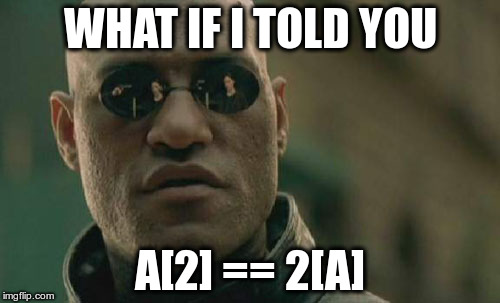
\includegraphics[width=0.8\textwidth]{\texDirectory/img/array.jpg}
	\end{figure}
\end{slide}

\section{Strings}

\begin{slide}
	\begin{block}{Definition}

	C does not provide a built-in data type for strings.
	A string is simply a sequence of characters terminated by a null character \alert{\texttt{\textbackslash 0}}.

	\begin{terminal}
	char string[6] = {'H', 'e', 'l', 'l', 'o', '\0'};
	\end{terminal}

	\end{block}
\end{slide}

\begin{slide}
	\begin{block}{String Literals}

	C provides built-in support for string literals.

	\begin{terminal}
	char string1[6] = {'H', 'e', 'l', 'l', 'o', '\0'};
	char string2[6] = "Hello";
	char string3[] = "Hello";
	\end{terminal}

	\end{block}
\end{slide}

\begin{slide}
	\begin{block}{Quiz}

	What is the output of the following program?

	\inputminted[
		fontsize=\scriptsize,
		firstline=10,
		linenos
	]{c}{\resDirectory/null.c}

	\pause

	\begin{terminal}
	Goodbye Good
	\end{terminal}

	\end{block}
\end{slide}

\begin{slide}
	\begin{block}{String Length vs. Array Length}

	Length of a string is defined as the number of characters before the null-terminator character.
	Size of a string is defined as the number of allocated bytes to it.

	\end{block}
\end{slide}

\begin{slide}
	\begin{block}{Quiz}

	What is the output of the following program?


	\inputminted[
		fontsize=\scriptsize,
		firstline=10,
		linenos
	]{c}{\resDirectory/strlen.c}

	\pause

	\begin{terminal}
	5 10
	\end{terminal}

	\end{block}
\end{slide}

\begin{slide}
	\begin{block}{\texttt{string.h} Library}

	The \texttt{string.h} library provides useful functions for string operations.

	\begin{columns}
	\column{0.5\textwidth}
	\begin{itemize}
	\item[] \texttt{strcat()}
	\item[] \texttt{strlen()}
	\item[] \texttt{strcpy()}
	\item[] ...
	\end{itemize}
	\column{0.5\textwidth}
	\begin{itemize}
	\item[] \texttt{strcmp()}
	\item[] \texttt{strtok()}
	\item[] \texttt{strstr()}
	\item[] ...
	\end{itemize}
	\end{columns}

	\end{block}
\end{slide}

\begin{slide}
	\begin{figure}
	
\includegraphics[width=0.8\textwidth]{\texDirectory/img/strncpy.jpg}
	\end{figure}
\end{slide}

\end{document}
